% OSGP
% Attacking smart meters and smart devices
% False data injection
% Disconnect attack
% Jamming


\begin{frame}{Principali vulnerabilità delle Smart Grid: attacchi e contromisure}
	\begin{itemize}[<+- | alert@+>]
		\item Digitalizzazione delle infrastrutture critiche
		\begin{itemize}
			\item Aggiunta capacità computazione e comunicazione
		\end{itemize}
		\item Dispositivi non critici e disconnessi
		\begin{itemize}
			\item Connessi $\rightarrow$ Dati \textsc{process-critical}
		\end{itemize}
		\item Anello debole della catena
		\begin{itemize}
			\item Smart Meter
		\end{itemize}
		\item Nuova sfida per i produttori
	\end{itemize}
\end{frame}

\begin{frame}{Principali vulnerabilità delle Smart Grid: sommario}
	\begin{itemize}
		\item Security Testing
		\item Open Smart Grid Protocol
		\item False Data Injection
		\item Disconnect Attack
		\item Jamming
	\end{itemize}
\end{frame}

\begin{frame}{Principali vulnerabilità delle Smart Grid: sommario}
	\begin{itemize}
		\alert<1>{\item Security Testing}
		\item Open Smart Grid Protocol
		\item False Data Injection
		\item Disconnect Attack
		\item Jamming
	\end{itemize}
\end{frame}

\begin{frame}{Principali vulnerabilità delle Smart Grid: dispositivi smart}
	\begin{block}{Smart Devices}
		\begin{itemize}
			\item Dispositivi capaci di computare e comunicare
			\item Godono di tutte le feature di un tipico dispositivo connesso alla rete
			\item Possono essere soggetti ad attacchi
		\end{itemize}
	\end{block}
\end{frame}

\begin{frame}{Principali vulnerabilità delle Smart Grid: Security Testing}
	\textbf{Institute for Security and Open Methodologies (ISECOM)}
	\begin{block}{Open Source Security Testing Methodology Manual (OSSTMM)}
		\begin{itemize}
			\item Information Security
			\item Process Security
			\item \textbf{Internet Technology Security}
			\item Communications Security
			\item Wireless Security
			\item Physical Security
		\end{itemize}
	\end{block}
\end{frame}


\begin{frame}{Principali vulnerabilità delle Smart Grid: Security Testing}
\begin{block}{Internet Technology Security}
	\begin{itemize}[<+- | alert@+>]
		\item Penetration Testing
		\begin{itemize}
			\item Kali Linux
		\end{itemize}
		\item Network Surveying
		\begin{itemize}
			\item Wireshark
		\end{itemize}
		\item Port Scanning, Services/System Identification, DoS Testing
		\begin{itemize}
			\item Nmap
		\end{itemize}
%		\item  Identification
%		\item System Identification
%		\begin{itemize}
%			\item Vulnerability Research and Verification
%		\end{itemize}
%		\item Denial of Service Testing
		\item Internet Application Testing
		\begin{itemize}
			\item Nessus
		\end{itemize}
		\item Exploit Testing
		\begin{itemize}
			\item Metasploit
		\end{itemize}
	\end{itemize}
\end{block}
\end{frame}

\begin{frame}{Principali vulnerabilità delle Smart Grid: sommario}
	\begin{itemize}
		\item Security Testing
		\alert<1>{\item Open Smart Grid Protocol}
		\item False Data Injection
		\item Disconnect Attack
		\item Jamming
	\end{itemize}
\end{frame}

\begin{frame}{Principali vulnerabilità delle Smart Grid: comunicazione tra data aggregator e smart meter}
	\begin{figure}[h] 
		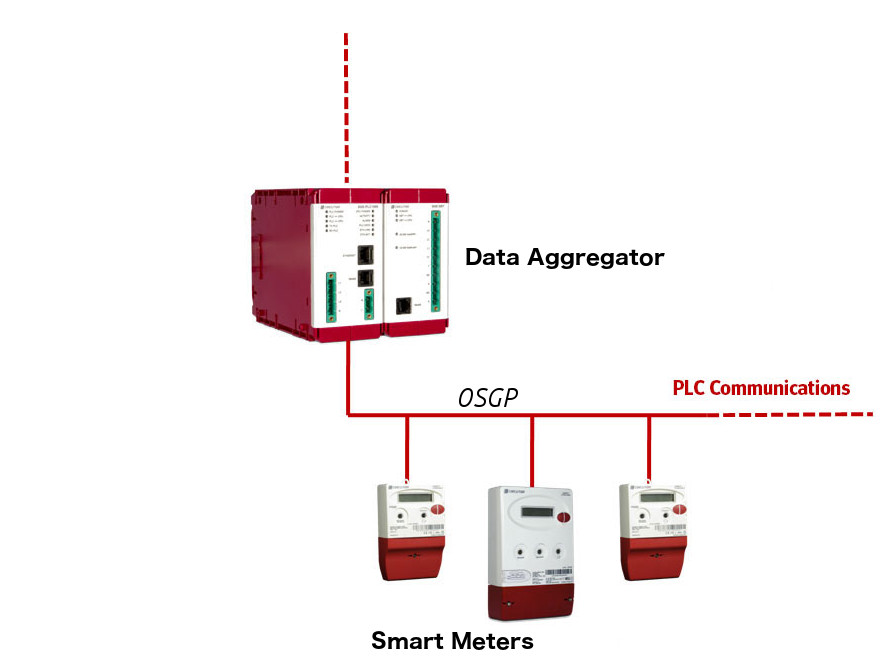
\includegraphics[scale=0.3,cfbox=blue_slides 1pt 0pt]{imgs/aggregator.jpg}
	\end{figure}
\end{frame}

\begin{frame}{Principali vulnerabilità delle Smart Grid: Open Smart Grid Protocol}
	\begin{itemize}[<+- | alert@+>]
		\item Sviluppato da European Telecommunications Standards Institute (ETSI), 2011
		\item Comunicazione su Powerline tra Data Concentrator (Aggregatore) e Smart meter
		\begin{itemize} 
			\item Protocollo Master-Slave: Master (Aggregatore) - Slave (Smart Meter)
			\item Ogni Aggregatore ha una zona di competenza a cui afferisce un certo numero di Smart Meter
		\end{itemize}
	\end{itemize}
	\begin{figure}[h] 
		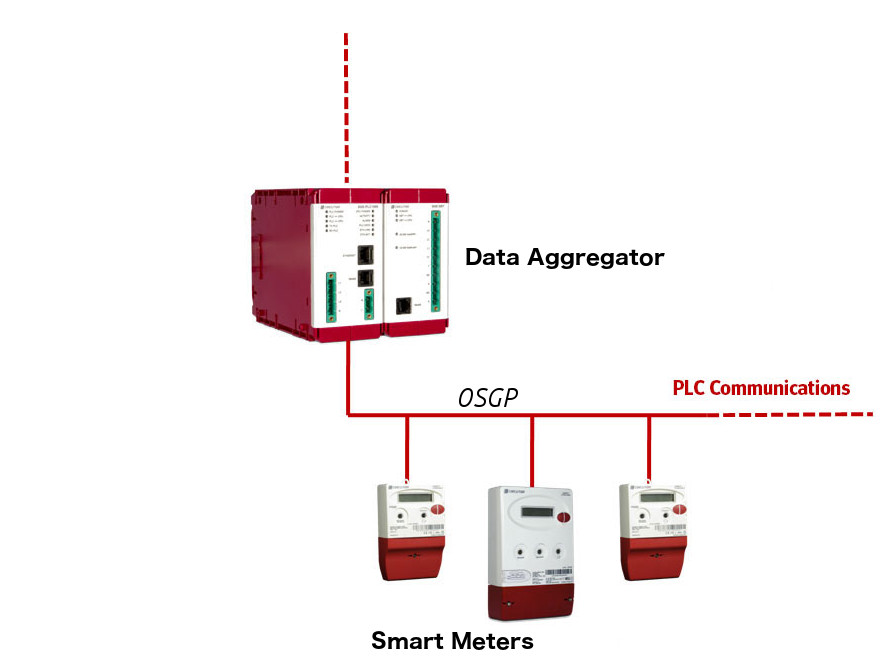
\includegraphics[scale=0.15,cfbox=blue_slides 1pt 0pt]{imgs/aggregator.jpg}
	\end{figure}
\end{frame}

\begin{frame}{Principali vulnerabilità delle Smart Grid: Open Smart Grid Protocol}
	\begin{itemize}[<+- | alert@+>]
		\item Fornisce meccanismi per proteggere la \emph{privacy} dei clienti
		\begin{itemize}[<+- | alert@+>]
			\item Restringendo l'accesso ai dati e cifrandoli evitando accessi non autorizzati
		\end{itemize}
		\item Costruito sullo stack protocollare ISO/IEC 14908-1
		\begin{itemize}[<+- | alert@+>]
			\item Fornisce servizi di autenticazione ma non garantisce \emph{confidentiality} dei dati
		\end{itemize}
		\item Migliora la sicurezza aggiungendo un proprio \emph{security layer}
		%che fornisce autenticazione e confidenzialità
	\end{itemize}
	\begin{figure}[h] 
		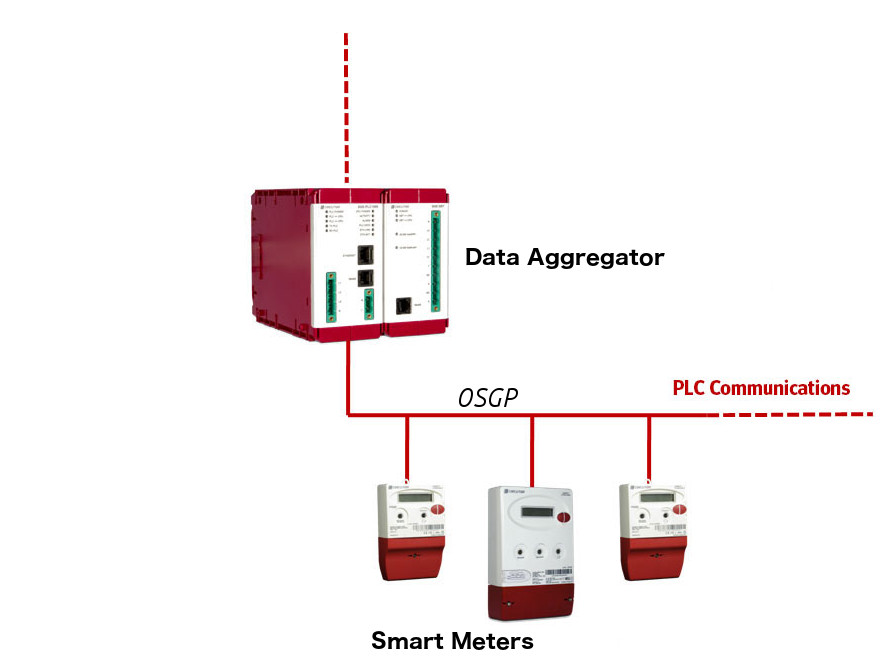
\includegraphics[scale=0.15,cfbox=blue_slides 1pt 0pt]{imgs/aggregator.jpg}
	\end{figure}
\end{frame}

\begin{frame}{Principali vulnerabilità delle Smart Grid: Open Smart Grid Protocol}
	\textbf{Fasi del protocollo OSGP}
	\begin{itemize}
		\item Setup
		\item Communication with Authenticated Encryption
	\end{itemize}
\end{frame}

\begin{frame}{Principali vulnerabilità delle Smart Grid: Open Smart Grid Protocol}
	\textbf{Fasi del protocollo OSGP}
	\begin{itemize}
		\alert<1>{\item Setup}
		\item Communication with Authenticated Encryption
	\end{itemize}
\end{frame}

\begin{frame}{Principali vulnerabilità delle Smart Grid: OSGP - Setup}
	\begin{itemize}[<+- | alert@+>]
		\item Processo di produzione del device OSGP
		\begin{itemize}
			\item Il dispositivo è configurato con una Open Media Access Key (OMAK) univoca a 96 bit
			%chiave principale/di riferimento del dispositivo
		\end{itemize}
		\item La chiave OMAK del device è consegnata alla società di servizi
		\item La società di servizi provvede a dotare il proprio Data Concentrator della chiave OMAK del dispositivo afferente alla zona di competenza
	\end{itemize}
\end{frame}
\begin{frame}{Principali vulnerabilità delle Smart Grid: OSGP - Setup}
	\begin{itemize}[<+- | alert@+>]
		\item Il Data Concentrator è in grado di rilevare ogni dispositivo a lui afferente grazie ad un processo di discovery
		\item Il Data Concentrator genera ed invia la Shared Key relativa alla sua zona di competenza ad ogni nuovo dispositivo scoperto
		\begin{itemize}
			\item Comunicazione cifrata utilizzando la OMAK del dispositivo
		\end{itemize}
		\item Ogni dispositivo rimpiazza la sua OMAK originaria con la Shared Key ricevuta
	\end{itemize}
\end{frame}
\begin{frame}{Principali vulnerabilità delle Smart Grid: Open Smart Grid Protocol}
	\textbf{Fasi del protocollo OSGP}
	\begin{itemize}
		\item Setup
		\alert<1>{\item Communication with Authenticated Encryption}
	\end{itemize}
\end{frame}

\begin{frame}{Principali vulnerabilità delle Smart Grid: OSGP - Communication with Authenticated Encryption}
	\begin{itemize}[<+- | alert@+>]
		\item Comunicazione iniziata dal Data Concentrator (Master)
		\item Data Concentrator invia messaggio di richiesta allo Smart Meter (Slave)
		\item Smart Meter decifra il messaggio, ne verifica l'autenticità e invia la risposta
		\item Richiesta e risposta cifrate con Shared Key
		\begin{itemize}
			\item Smart Meter e Data Concentrator sono identificati dai campi Subnet e Node ID del pacchetto di richiesta/risposta
		\end{itemize}
	\end{itemize}
\end{frame}

\begin{frame}{Principali vulnerabilità delle Smart Grid: OSGP - Authenticated Encryption Scheme}
	\textbf{Schema di cifratura}
	\begin{figure}[h] 
		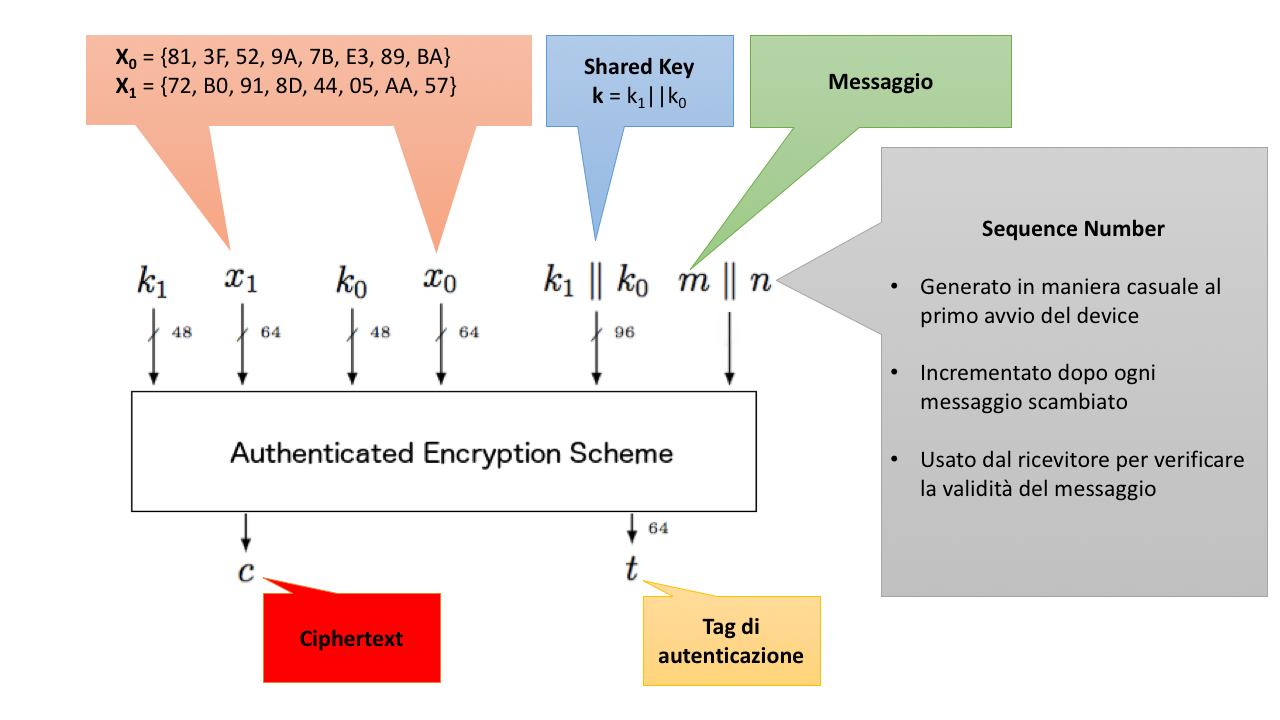
\includegraphics[scale=0.3,cfbox=blue_slides 1pt 0pt]{imgs/schemes/blackbox-1.png}
		%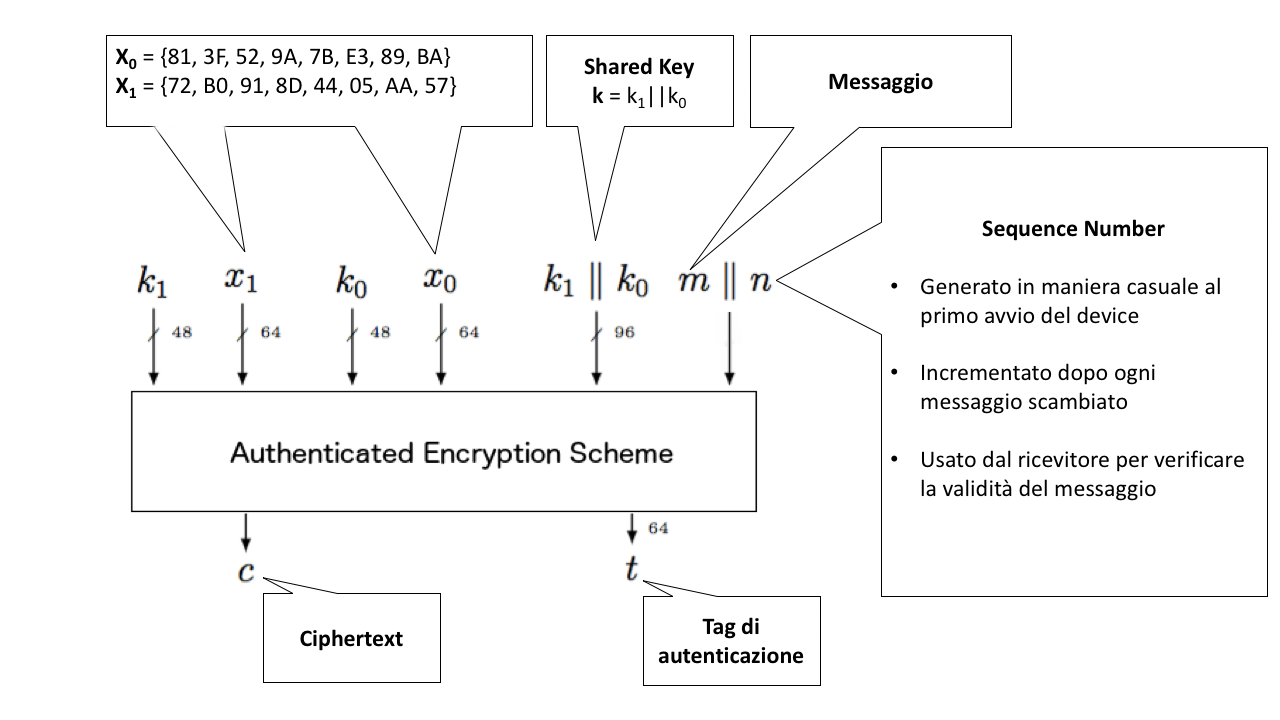
\includegraphics[scale=0.3,cfbox=blue_slides 1pt 0pt]{imgs/schemes/blackbox-1bw.png}
	\end{figure}
\end{frame}

\begin{frame}{Principali vulnerabilità delle Smart Grid: OSGP - Authenticated Encryption Scheme}
	\textbf{Schema di cifratura}
	\begin{figure}[h] 
		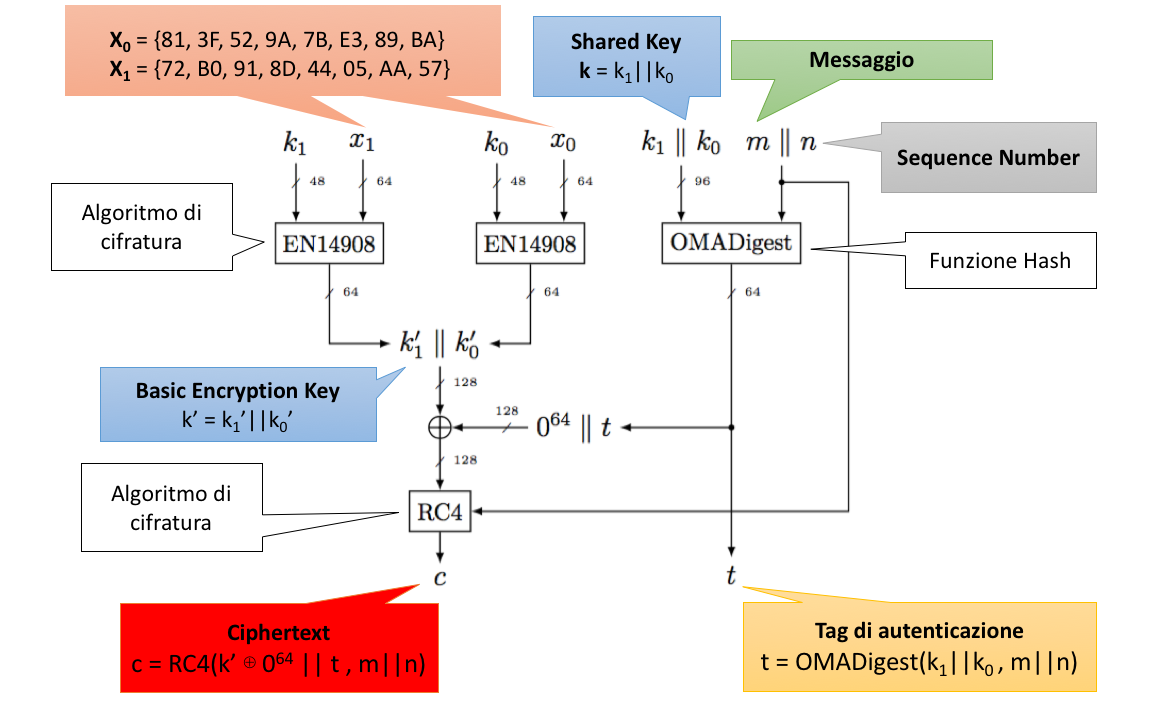
\includegraphics[scale=0.3,cfbox=blue_slides 1pt 0pt]{imgs/schemes/scheme-1(info).png}
		%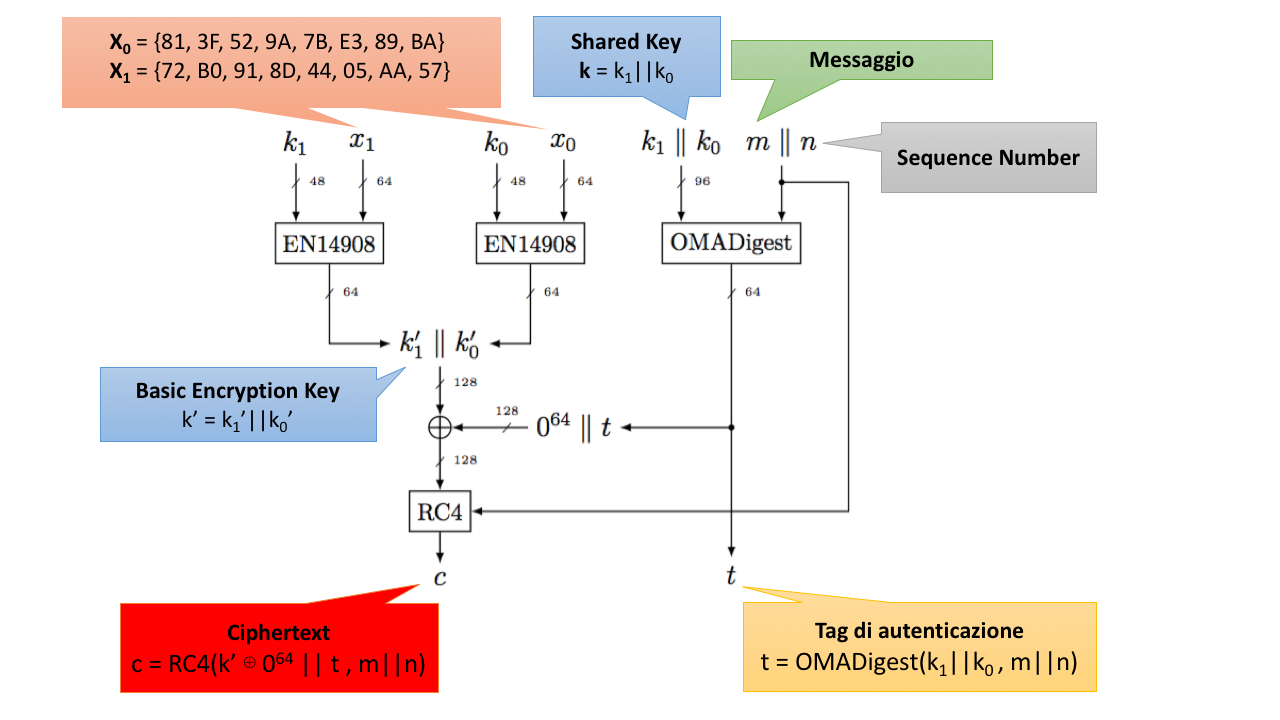
\includegraphics[scale=0.3,cfbox=blue_slides 1pt 0pt]{imgs/schemes/scheme-1.png}
		%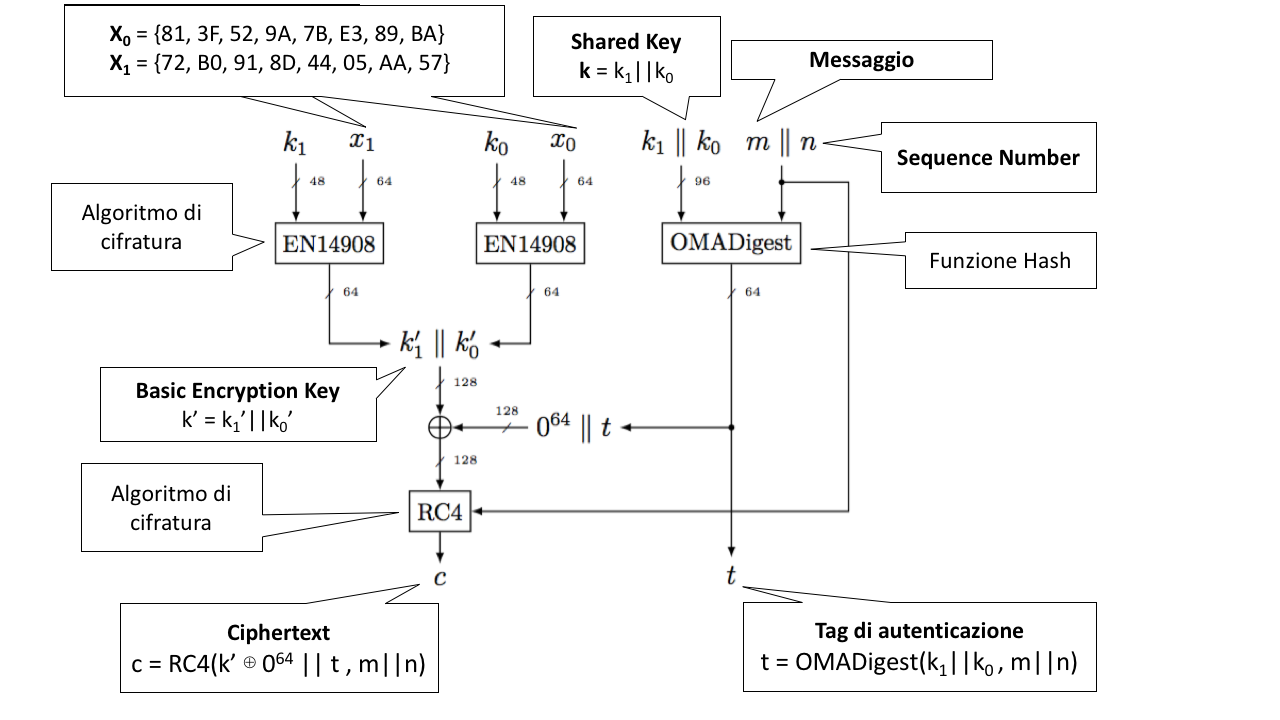
\includegraphics[scale=0.3,cfbox=blue_slides 1pt 0pt]{imgs/schemes/scheme-1bw(info).png}
		%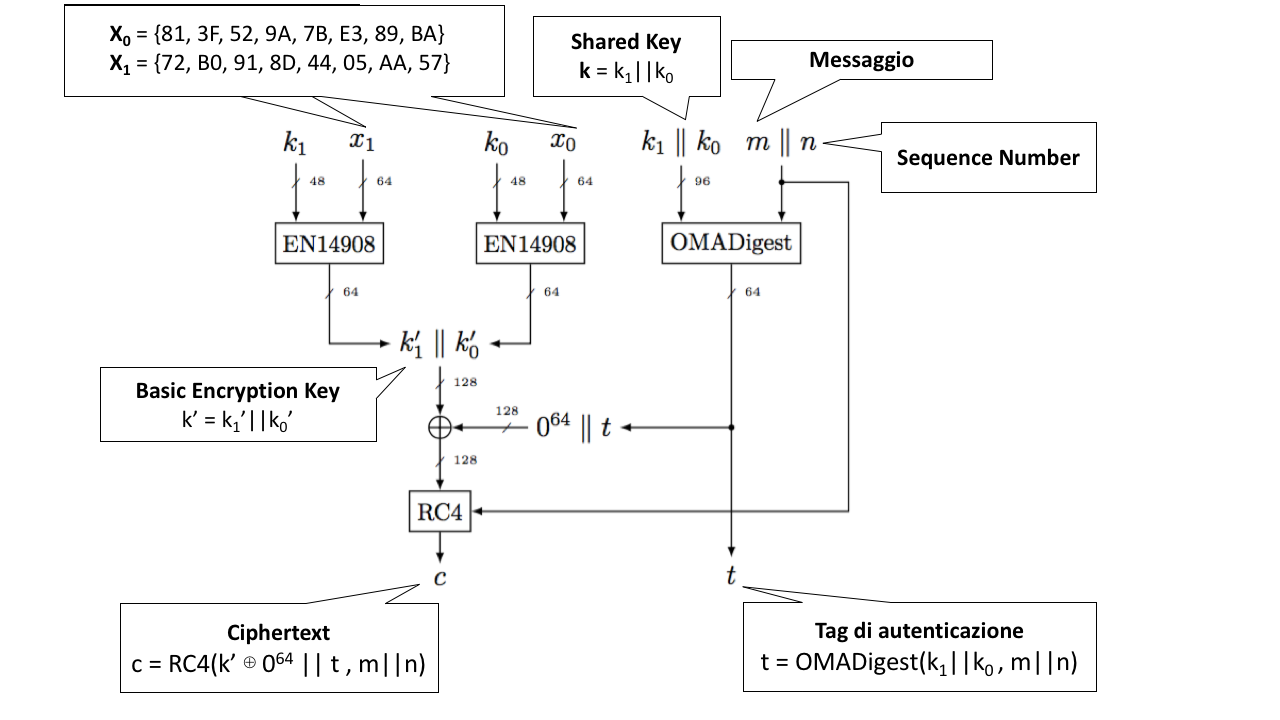
\includegraphics[scale=0.3,cfbox=blue_slides 1pt 0pt]{imgs/schemes/scheme-1bw.png}
	\end{figure}
\end{frame}

%\begin{frame}{Principali vulnerabilità delle Smart Grid: OSGP - Authenticated Encryption Scheme}
%	\textbf{Schema di cifratura: parametri di input}
%	\begin{figure}[h] 
%		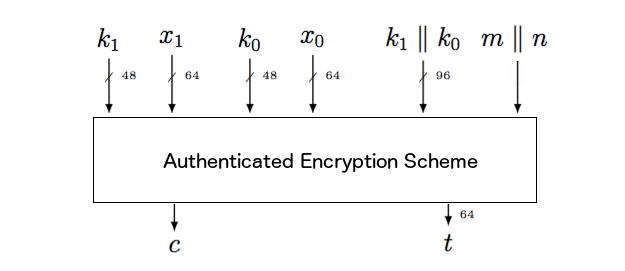
\includegraphics[scale=0.25,cfbox=blue_slides 1pt 0pt]{imgs/c_scheme.png}
%	\end{figure}
%		\only<1>{Costanti
%		\begin{itemize}
%			\item $x_0 = \{${\tt 81, 3F, 52, 9A, 7B, E3, 89, BA}$\}$
%			\item $x_1 = \{${\tt 72, B0, 91, 8D, 44, 05, AA, 57}$\}$
%		\end{itemize}}
%		\only<2>{Shared Key $k = k_1 \| k_0$
%		\begin{itemize}
%			\item $k$
%			\item $k_1$
%			\item $k_0$
%		\end{itemize}}
%		\only<3>{Messaggio $m$}
%		\only<4>{Sequence number $n$
%			\begin{itemize}
%				\item Generato in maniera casuale al primo avvio del device
%				\item Incrementato dopo ogni messaggio scambiato
%				\item Inviato insieme al messaggio
%				%\item Utilizzato nella funzione OMADigest
%				\item Usato dal ricevitore per verificare la validità del messaggio
%				\begin{itemize}
%					\item Messaggio valido se $n$ ricevuto $\in [n-1, n+8]$
%					\item In caso contrario, il ricevitore invia messaggio cifrato contenente il sequence number $n$ corrente del device
%				\end{itemize}
%			\end{itemize}}
%\end{frame}

%\begin{frame}{Principali vulnerabilità delle Smart Grid: OSGP - Authenticated Encryption Scheme}
%	\textbf{Schema di cifratura: parametri di output}
%	\begin{figure}[h] 
%		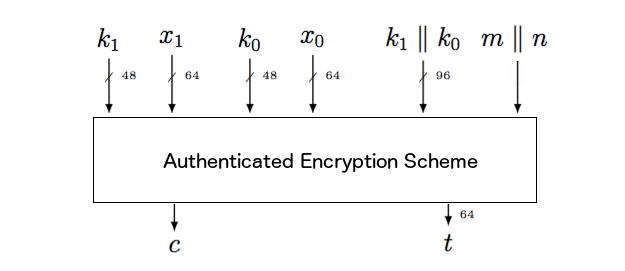
\includegraphics[scale=0.25,cfbox=blue_slides 1pt 0pt]{imgs/c_scheme.png}
%	\end{figure}
%		\only<1>{Tag di autenticazione $t$}
%		\only<2>{Ciphertext $c$}
%\end{frame}

%\begin{frame}{Principali vulnerabilità delle Smart Grid: OSGP - Authenticated Encryption Scheme}
%	\textbf{Parametri di input dello schema di cifratura}
%	\begin{itemize}
%		\item Costanti
%		\begin{itemize}
%			\item $x_0 = \{${\tt 81, 3F, 52, 9A, 7B, E3, 89, BA}$\}$, 64 bit
%			\item $x_1 = \{${\tt 72, B0, 91, 8D, 44, 05, AA, 57}$\}$, 64 bit
%		\end{itemize}
%		\pause
%		\item Shared Key $k = k_1 \| k_0$
%		\begin{itemize}
%			\item $k$, 96 bit
%			\item $k_1$, 48 bit
%			\item $k_0$, 48 bit
%		\end{itemize}
%	\end{itemize}
%\end{frame}

%\begin{frame}{Principali vulnerabilità delle Smart Grid: OSGP - Authenticated Encryption Scheme}
%	\textbf{Parametri di input dello schema di cifratura}
%	\begin{itemize}[<+- | alert@+>]
%		\item Messaggio $m$
%		\item Sequence number $n$
%		\begin{itemize}
%			\item Generato in maniera casuale al primo avvio del device
%			\item Incrementato dopo ogni messaggio scambiato
%			\item Inviato insieme al messaggio
%			%\item Utilizzato nella funzione OMADigest
%			\item Usato dal ricevitore per verificare la validità del messaggio
%			\begin{itemize}
%				\item Messaggio valido se $n$ ricevuto $\in [n-1, n+8]$
%				\item In caso contrario, il ricevitore invia messaggio cifrato contenente il sequence number $n$ corrente del device
%			\end{itemize}
%		\end{itemize}
%	\end{itemize}
%\end{frame}

%\begin{frame}{Principali vulnerabilità delle Smart Grid: OSGP - Authenticated Encryption Scheme}
%	\textbf{Parametri di output dello schema di cifratura}
%	\begin{itemize}
%		\item Tag di autenticazione $t$% \gets OMADigest(k_1\|k_0,\,m\|n)$, 64 bit
%		\item Ciphertext $c$% \gets RC4(k^{\prime} \oplus 0^{64}\|t,\,m\|n)$
%	\end{itemize}
%\end{frame}

%\begin{frame}{Principali vulnerabilità delle Smart Grid: OSGP - Authenticated Encryption Scheme}
%	\textbf{Building Blocks dello schema di cifratura autenticata}
%	\begin{itemize}
%		\item Protocollo EN14908
%		\item Funzione OMADigest
%		\item Algoritmo di cifratura RC4
%	\end{itemize}
%\end{frame}

%\begin{frame}{Principali vulnerabilità delle Smart Grid: OSGP - Authenticated Encryption Scheme}
%	\textbf{Building Blocks dello schema di cifratura autenticata}
%	\begin{itemize}
%		\alert<1>{\item Protocollo EN14908}
%		\item Funzione OMADigest
%		\item Algoritmo di cifratura RC4
%	\end{itemize}
%\end{frame}

%\begin{frame}{Principali vulnerabilità delle Smart Grid: OSGP - Authenticated Encryption Scheme}
%	\textbf{Protocollo EN14908}\\
%	Setup iniziale con valore scelto in maniera casuale
%	\begin{figure}[h] 
%		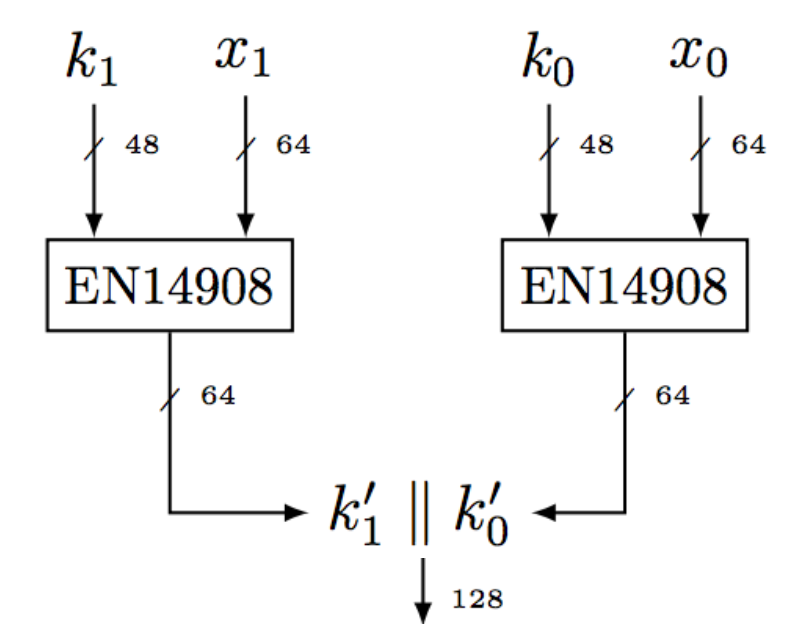
\includegraphics[scale=0.3,cfbox=blue_slides 1pt 0pt]{imgs/EN14908.png}
%	\end{figure}
%	Base Encryption Key (BEK) $k^{\prime} = k_1^{\prime} \| k_0^{\prime}$
%		\begin{itemize}
%			\item $k^{\prime}$, 128 bit
%			\item $k_1^{\prime} \gets EN14908(k_1,\,x_1)$, 64 bit
%			\item $k_0^{\prime} \gets EN14908(k_0,\,x_0)$, 64 bit
%		\end{itemize}
%\end{frame}

%\begin{frame}{Principali vulnerabilità delle Smart Grid: OSGP - Authenticated Encryption Scheme}
%	\textbf{Building Blocks dello schema di cifratura autenticata}
%	\begin{itemize}
%		\item Protocollo EN14908
%		\alert<1>{\item Funzione OMADigest}
%		\item Algoritmo di cifratura RC4
%	\end{itemize}
%\end{frame}

%\begin{frame}{Principali vulnerabilità delle Smart Grid: OSGP - Authenticated Encryption Scheme}
%	\textbf{Funzione OMADigest}
%	\begin{figure}[h] 
%		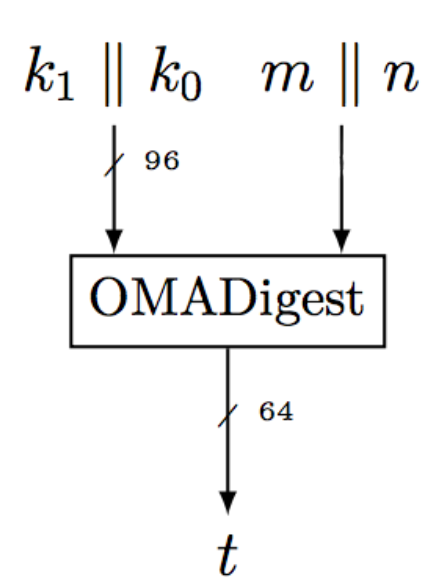
\includegraphics[scale=0.4,cfbox=blue_slides 1pt 0pt]{imgs/OMADigest.png}
%	\end{figure}
%	\begin{itemize}
%		\item Messaggio $m$
%		\item Sequence number $n$
%		\item Shared Key $k = k_1 \| k_0$
%	\end{itemize}
%\end{frame}

%\begin{frame}{Principali vulnerabilità delle Smart Grid: OSGP - Authenticated Encryption Scheme}
%	\textbf{Building Blocks dello schema di cifratura autenticata}
%	\begin{itemize}
%		\item Protocollo EN14908
%		\item Funzione OMADigest
%		\alert<1>{\item Algoritmo di cifratura RC4}
%	\end{itemize}
%\end{frame}

%\begin{frame}{Principali vulnerabilità delle Smart Grid: OSGP - Authenticated Encryption Scheme}
%	\textbf{Algoritmo di cifratura RC4}
%	\begin{itemize}[<+- | alert@+>]
%		\item Stream cipher RC4 - Ron Rivest, 1987 (mai pubblicato uff.)
%		\begin{itemize}
%			\item Periodicità nei primi 256 byte
%			\item Forte correlazione fra chiave e keystream (\textit{Breaking 104 bit WEP in less than 60 seconds})
%		\end{itemize}
%	\end{itemize}
%\end{frame}


%\begin{frame}{Principali vulnerabilità delle Smart Grid: OSGP - Authentication}
%	\begin{itemize}[<+- | alert@+>]
%		\item Data concentrator utilizza autenticazione basata su digest a livello applicativo per autenticare messaggi tra i dispositivi
%		\item Viene aggiunto ai messaggi un \emph{sequence number} e se ne effettua il digest, evitando così \emph{replay attack}
%		\item Ogni device sceglie un sequence number $N$ ed accetta solo messaggi aventi sequence number compreso tra $N-1$ e $N+8$
%		% per i restanti manda una response NACK contenente il messaggio "invalid sequence number" seguita dal sequence number desiderato -> il data concentrator deve usare tale numero
%		\item Tutti i dati dei device sono protetti dall’autenticazione basata su digest al livello applicativo sia per operazioni di lettura che di scrittura
%		%include: Configurazione di un dispositivo OSGP, Fatturazioni e profili di carico OSGP, Richieste di cancellazione del carico, Time setting
%
%	\end{itemize}
%\end{frame}

%\begin{frame}{Principali vulnerabilità delle Smart Grid: OSGP - Authentication}
%	\textbf{Request}\newline
%		Formato
%		\begin{figure}[t]
%		
\includegraphics[scale=0.35,cfbox=blue_slides 1pt 0pt]{imgs/req1.png}
%		\end{figure}
%		\pause
%		Digest con OMAK su
%		\begin{figure}[t]
%			
\includegraphics[scale=0.35,cfbox=blue_slides 1pt 0pt]{imgs/req2.png}
%		\end{figure}
%\end{frame}
%
%\begin{frame}{Principali vulnerabilità delle Smart Grid: OSGP - Authentication}
%	\textbf{Response}\newline
%		Formato
%		\begin{figure}[t]
%			
\includegraphics[scale=0.35,cfbox=blue_slides 1pt 0pt]{imgs/res1.png}
%		\end{figure}
%		\pause
%		Digest con OMAK su
%		\begin{figure}[t]
%			
\includegraphics[scale=0.28,cfbox=blue_slides 1pt 0pt]{imgs/res2.png}
%		\end{figure}
%\end{frame}

% Subnet e Node si riferiscono sempre a subnet/node del target della richiesta. Stesso indirizzo in entrambe le direzioni. 
% Request e Sequence fanno riferimento sempre ai valori nel messaggio di richiesta originale.

%\begin{frame}{Principali vulnerabilità delle Smart Grid: OSGP - Authenticated Encryption Scheme}
%	\begin{figure}[t]
%		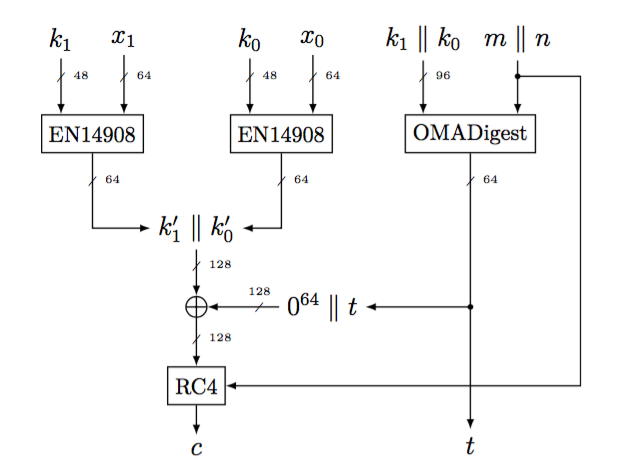
\includegraphics[scale=0.35,cfbox=blue_slides 1pt 0pt]{imgs/osgp.png}
%	\end{figure}
%	{$t \gets OMADigest(k_1\|k_0,\,m\|n)$, 64 bit}\\
%	{$c \gets RC4(k^{\prime} \oplus 0^{64}\|t,\,m\|n)$}
%	\only<1>{Costante $x_0 = \{${\tt 81, 3F, 52, 9A, 7B, E3, 89, BA}$\}$}
%	\only<2>{Costante $x_1 = \{${\tt 72, B0, 91, 8D, 44, 05, AA, 57}$\}$}
%	\only<3>{Open Media Access Key (OMAK) univoca per dispositivo: $k = k_1 \| k_0$}
%	\only<4>{$m$: messaggio}
%	\only<5>{$n$: numero di sequenza}
%	\only<6>{$t$: tag di autenticazione}
%	\only<7>{Base Encryption Key (BEK) $k^\prime = k^{\prime}_{1} \| k^{\prime}_{0}$}
%	\only<8>{$c$: ciphertex}
%\end{frame}

%\begin{frame}{Principali vulnerabilità delle Smart Grid: Analisi di OSGP}
%	\textbf{Problemi legati alla sicurezza di OSGP}	
%	\begin{itemize}[<+- | alert@+>]
%		\item OSGP utilizza RC4
%		\begin{itemize}
%			\item L'algoritmo RC4 soggetto ad attacchi di \emph{statistical key recovery} e \emph{plaintext key recovery}
%		\end{itemize}			
%		\item Esiste un algoritmo in grado di invertire la funzione OMADigest
%		\item Chiavi di sessione derivate dalla Shared Key
%			\begin{itemize}
%				\item Determinati attacchi permettono di recuperare la Shared Key
%			\end{itemize}
%	\end{itemize}	
%\end{frame}

\begin{frame}{Principali vulnerabilità delle Smart Grid: sommario}
	\begin{itemize}
		\item Security Testing
		\item Open Smart Grid Protocol
		\alert<1>{\item False Data Injection}
		\item Disconnect Attack
		\item Jamming
	\end{itemize}
\end{frame}

\begin{frame}{Principali vulnerabilità delle Smart Grid: False Data Injection}
	\begin{itemize}[<+- | alert@+>]
		\item Scambio informazioni stato
		\item Stima dello stato $\rightarrow$ Modello \textit{real-time}
		\item Manomettere le misure
		\begin{itemize}
			\item Frode
			\item Sovraccaricare l'infrastruttura
			\item Manipolare prezzi di mercato
		\end{itemize}
		\item \textit{Bad Data Injection}
		\begin{itemize}
			\item Rilevabile
		\end{itemize}
		\item \textit{Stealth Bad Data Injection}
		\begin{itemize}
			\item Non rilevabile
			\item Necessaria conoscenza della topologia
			\item Possibile inferire i parametri legati alla topologia
			\begin{itemize}
				\item \textit{Linear Independent Component Analysis}
			\end{itemize}
		\end{itemize}
	\end{itemize}
\end{frame}
% opzionale %%%%%%%%%%%%%%%%%%%%%%%%%%%%%%%%%%%%%%%%%%%%%%%%%%%%%%%%%%%%%%%%%%%%%
\begin{frame}{Principali vulnerabilità delle Smart Grid: attacchi e contromisure}
\textbf{Modello Matematico}
	\begin{block}{Vettore delle misurazioni} % vorrei mettere tipo l'alert
		$\textbf{z} = \textbf{h(x)} + \textbf{e}$
		\begin{itemize}
			\item $\textbf{h(x)}$: relazione non lineare tra le misure $\textbf{z}$ e lo stato del sistema $\textbf{x}$
			\item $\textbf{e} = [e_1, \ldots, e_m]^T$, rumore Gaussiano delle misure
		\end{itemize}
	\end{block}
	\pause
	\begin{block}{Modello di approssimazione lineare della misura di corrente}
		Misura sotto Operazioni Normali: $\textbf{z} =  \textbf{Hx} + \textbf{e}$
		\begin{itemize}
			\item Vettore di stato stimato: $\widehat{\textbf{x}} = (\textbf{H}^T\sum_e^{-1}\textbf{H})-1\textbf{H}^T\sum_e^{-1}\textbf{z}$
			\item $\textbf{H} \in {\rm I\!R}$, definito come
			\begin{itemize}
				\item $\textbf{H}=\frac{\partial\textbf{h(x)}}{\partial\textbf{x}}|_{x=0}$
			\end{itemize}
			\item Matrice di covarianza $\Sigma_e$
		\end{itemize}
	\end{block}
\end{frame}

\begin{frame}{Principali vulnerabilità delle Smart Grid: attacchi e contromisure}
	\textbf{Modello Matematico}
	\begin{itemize}
	\item Bad Data Injection
	\begin{itemize}
		\item Misura sotto attacco non stealth: $\textbf{z}^\prime = \textbf{H}(\textbf{x}) + \textbf{b} + e$
		\item Vettore residuo: $\textbf{r} = \textbf{z} - \textbf{H}\widehat{\textbf{x}}$
		\item Rilevamento bad data: $max_i(|\textbf{r}_i|/\sqrt{cov(\textbf{r})}) \geq \gamma$
	\end{itemize}
	\item Stealth Bad Data Injection
	\begin{itemize}
		\item Misura sotto attacco stealth: $\textbf{z}^\prime = \textbf{H}(\textbf{x} + \delta\textbf{x}) + e$
		\item Non rilevabile usando meccanismi a soglia
	\end{itemize}
\end{itemize}
\let\thefootnote\relax\footnote{$\textbf{H}(\textbf{x})$ e $\textbf{H}(\textbf{x} + \delta\textbf{x})$ sono prodotti $matrice \times vettore$}
\end{frame}
%%%%%%%%%%%%%%%%%%%%%%%%%%%%%%%%%%%%%%%%%%%%%%%%%%%%%%%%%%%%%%%%%%%%%%%%%%%%%%%%%

\begin{frame}{Principali vulnerabilità delle Smart Grid: sommario}
	\begin{itemize}
		\item Security Testing
		\item Open Smart Grid Protocol
		\item False Data Injection
		\alert<1>{\item Disconnect Attack}
		\item Jamming
	\end{itemize}
\end{frame}

\begin{frame}{Principali vulnerabilità delle Smart Grid: Disconnect Attack}
	\begin{itemize}[<+- | alert@+>]
		\item Remote Connect Disconnect (RCD)
		\item Attacco RCD $\rightarrow$ Blackout/Danni alla rete
		\item Difesa: ritardi casuali nell'esecuzione dei comandi RCD
		\begin{itemize}
			\item Prevenire rapidi cambiamenti del carico elettrico
			\item Tempo per rilevare e fermare un attacco in corso
		\end{itemize}
	\end{itemize}
\end{frame}

\begin{frame}{Principali vulnerabilità delle Smart Grid: sommario}
	\begin{itemize}
		\item Security Testing
		\item Open Smart Grid Protocol
		\item False Data Injection
		\item Disconnect Attack
		\alert<1>{\item Jamming}
	\end{itemize}
\end{frame}

\begin{frame}{Principali vulnerabilità delle Smart Grid: Jamming}
	\begin{block}{}
	Strategia d'attacco utilizzata per la manipolazione del mercato elettrico
	\end{block}
	\pause
	\begin{block}{Assunzione}
	Si utilizza un sistema di comunicazione wireless, come \textbf{\color{blue_slides}WiMAX}, per effettuare il broadcast delle informazioni relative ai prezzi
	\end{block}
\end{frame}

\begin{frame}{Principali vulnerabilità delle Smart Grid: Jamming}
	\textbf{Attacco}\\
	{\small [Li, Husheng, and Zhu Han. ``Manipulating the electricity power market via jamming the price signaling in smart grid.'' \emph{GLOBECOM Workshops (GC Wkshps), 2011 IEEE}. IEEE, 2011.]}
	\begin{enumerate}[<+- | alert@+>]
		\item L'attaccante fa Jamming in un'area molto popolata
		\item L'utente rimane a conoscenza del vecchio prezzo della corrente
		\item L'attaccante monitora il mercato elettrico
		\item Quando il prezzo cambia significativamente, si smette di fare Jamming
		\item Ogni utente adatta il proprio consumo energetico in base al nuovo prezzo
		%se il nuovo prezzo è superiore, l'utente diminuisce i consumi, facendo calare il prezzo con p alta. se il nuovo prezzo è più piccolo, l'utente incrementa i consumi, aumentando con alta probabilità il prezzo.
		\item L'attaccante può avere profitti da questa manipolazione del mercato
		%è in grado di predire come si comporteranno gli utenti alla ricezione del nuovo prezzo e quindi sono in grado di cambiare il prezzo della corrente quando e come vogliono.
	\end{enumerate}
\end{frame}

\begin{frame}{Principali vulnerabilità delle Smart Grid: Jamming}
	\begin{block}{Contromisure}
		Evitare di modificare il consumo di energia in maniera simultanea.\newline
		\textbf{\color{blue_slides}IDEA: si utilizza uno schema di \emph{backoff}} 
	\end{block}
	\pause
	\begin{block}{}
	Ogni consumer sceglie un tempo casuale per cambiare la propria power response evitando che l'attaccante possa predire il comportamento dell'utente e quindi capire in che modo varia il prezzo della corrente
		%randomness: perchè i consumi sono in base alle esigenze e tendono a variare da persona a persona
		%utilizzando backoff casuali per evitare collisioni dovute a trasmissioni simultanee
		%schema di backoff casuale: un consumer sceglie un tempo casuale per cambiare la propria power response
		%si diffondono info relative ai cambiamenti in un intervallo di tempo piu ampio cosicchè la randomness del mercato possa contrattaccare i cambiamenti dei jammed user
	\end{block}
\end{frame}